\documentclass[10pt,a4paper, margin=1in]{article}
\usepackage{fullpage}
\usepackage{relsize}
\usepackage{amsfonts, amsmath, pifont}
\usepackage{amsthm}
\usepackage{graphicx}
\usepackage{float}

\usepackage{tkz-euclide}
\usepackage{tikz}
\usepackage{pgfplots}
\pgfplotsset{compat=1.13}
\begin{filecontents}{q1.dat}





 n   xn 
 0   1
 1   -0.5  
 2   0
 3   -0.5
\end{filecontents}

\begin{filecontents}{q2.dat}
 n   xn 
 0   0.75
 1   0.56  
 2   0.25
 3   0.56
\end{filecontents}



\usepackage{geometry}
 \geometry{
 a4paper,
 total={210mm,297mm},
 left=10mm,
 right=10mm,
 top=10mm,
 bottom=10mm,
 }
 % Write both of your names here. Fill exxxxxxx with your ceng mail address.
 \author{
  OREN, Zeki\\
  \texttt{e2264612@ceng.metu.edu.tr}
  \and
  KOSEN, Emrah\\
  \texttt{e1942317@ceng.metu.edu.tr}
}
\title{CENG 384 - Signals and Systems for Computer Engineers \\
Spring 2018-2019 \\
Written Assignment 4}
\begin{document}
\maketitle



\noindent\rule{19cm}{1.2pt}

\begin{enumerate}

\item 
    \begin{enumerate}
    % Write your solutions in the following items.
    \item %write the solution of q1a
    
    
    y[n] = 2x[n] - $\dfrac{1}{8}$y[n-2] + $\dfrac{3}{4}$y[n-1]\\\\\\
    $\dfrac{1}{8}$y[n-2] - $\dfrac{3}{4}$y[n-1] + y[n]  = 2x[n] \\\\\\\\
   
   \item %write the solution of q1b
   
    x[n] = $e^{jwn}$\\
    
     y[n] = $H(jw).e^{jwn}$\\\\\\
      $\dfrac{1}{8}$ $H(jw).e^{jw(n-2)}$ - $\dfrac{3}{4}H(jw).e^{jw(n-1)}$ + $H(jw).e^{jwn}$  = 2$e^{jwn}$ \\\\\\
      $\dfrac{1}{8}$ $H(jw).e^{-2jw}$ - $\dfrac{3}{4}H(jw).e^{-jw}$ + $H(jw)$  = 2 \\\\\\
       H(jw).($\dfrac{1}{8}e^{-2jw} - \dfrac{1}{8}e^{-jw} + 1$ )   = 2 \\\\\\
        H(jw) = $\dfrac{2}{\dfrac{1}{8}e^{-2jw} - \dfrac{3}{4}e^{-jw} + 1} $  \\\\\\\\
       
      
    
    
    
    
    
    \item %write the solution of q1c 
    H(jw) = $\dfrac{2}{\dfrac{1}{8}e^{-2jw} - \dfrac{3}{4}e^{-jw} + 1} $  \\\\\\
    H(jw) = $\dfrac{-2}{1 - \dfrac{1}{4}e^{-jw}} + \dfrac{4}{1 - \dfrac{1}{2}e^{-jw}} $ \\\\\\
    h[n] = $-2(\dfrac{1}{4})^nu[n] + 4 (\dfrac{1}{2})^nu(n)$ \\\\\\
    
    \newpage
    \item %write the solution of q1d 
    y[n] = x[n]*h[n]\\\\
    $X(e^{jw}) = \dfrac{1}{1- \dfrac{1}{4}e^{-jw}}$\\\\\\
    $Y(e^{jw}) = X(e^{jw}).H(e^{jw}) $\\\\
    = $ \dfrac{1}{1- \dfrac{1}{4}e^{-jw}} . (\dfrac{-2}{1 - \dfrac{1}{4}e^{-jw}} + \dfrac{4}{1 - \dfrac{1}{2}e^{-jw}})$\\\\\\
    $ -2.(\dfrac{1}{1- \dfrac{1}{4}e^{-jw}})^{2}  +   \dfrac{4}{ (1- \dfrac{1}{4}e^{-jw}).(1 - \dfrac{1}{2}e^{-jw})}$\\\\\\
    $ -2.(\dfrac{1}{1- \dfrac{1}{4}e^{-jw}})^{2}  +   \dfrac{32}{ (4 - e^{-jw}).(2 - e^{-jw})}$\\\\\\
    $\dfrac{32}{(4 - e^{-jw}).(2 - e^{-jw})}$ = $\dfrac{A}{(4 - e^{-jw})}$ + $\dfrac{B}{(2 - e^{-jw})}$ = $\dfrac{-16}{(4 - e^{-jw})}$ + $\dfrac{16}{(2 - e^{-jw})}$\\\\\\
    
    $Y(e^{jw}) = -2.(\dfrac{1}{1- \dfrac{1}{4}e^{-jw}})^{2} + -4(\dfrac{1}{1 - \dfrac{1}{4}e^{-jw}}) + 8(\dfrac{1}{1 - \dfrac{1}{2}e^{-jw}})$\\\\\\
   
    y[n] = -2.(n + 1).$(\dfrac{1}{4})^{n}$u[n] - 4$(\dfrac{1}{4})^{n}$u[n] + 8$(\dfrac{1}{2})^{n}$u[n]\\\\\\\\
    
    

    \end{enumerate}


\item %write the solution of q2

    % Write your solutions in the following items.
    $H_{1}(jw)$ = $\dfrac{1}{1 - \dfrac{1}{3}e^{-jw}}$ + $H_{2}(jw)$ \\\\\\
    = $\dfrac{5e^{-jw} - 12}{e^{-2jw} -7e^{-jw} +12}$ \\\\\\
    = $\dfrac{5e^{-jw} - 12}{(e^{-jw} - 4).(e^{-jw} - 3)}$ \\\\\\
    = $\dfrac{A}{(e^{-jw} - 4)}$ + $\dfrac{B}{(e^{-jw} - 3)}$ \\\\\\
    = $\dfrac{8}{(e^{-jw} - 4)}$ - $\dfrac{3}{(e^{-jw} - 3)}$ \\\\\\
    = $\dfrac{-2}{(1 - \dfrac{1}{4}e^{-jw})}$ + $\dfrac{1}{(1 -\dfrac{1}{3}e^{-jw})}$\\\\\\
     h[n] = -2($\dfrac{1}{4})^n$u[n] + ($\dfrac{1}{3})^n$u[n]\\\\\\
     h[n] = $ h_{1}[n] + h_{2}[n]$ = -2($\dfrac{1}{4})^n$u[n] + ($\dfrac{1}{3})^n$u[n]\\\\\\
     h[n] = $ h_{1}[n] + h_{2}[n]$ = -2($\dfrac{1}{4})^n$u[n] +  $ h_{2}[n]$\\\\
     $h_{2}[n]$ = -2($\dfrac{1}{4})^n$u[n]\\
     
     
\item %write the solution of q3
\begin{enumerate}
    \item %write the solution of q3a
        
    x(t) = $\dfrac{sin(2\pi t)}{\pi t} +cos(3\pi t)$\\\\
    X(jw) = $\pi (\delta$(w-3$\pi$) + $\delta$(w+3 $\pi$)) + 2rect(w)\\\\
    
  \begin{tikzpicture}
    \def\x{1} % replace 1 with desired value here
    \draw[-latex] (0,0) -- ++(-3,0);
    \draw[-latex] (0,0) -- ++(3,0)  node[right]{$w$};
    \draw[-latex] (0,0) -- ++(0,3.0\x)node[above]{$X(jw)$};
    \draw[] (0,0) -- ++(0,1.2\x)node[left]{2};
    \draw[] (-2,0) -- ++(0,0)node[below]{-3$\pi$};
    \draw[] (2,0) -- ++(0,0)node[below]{3$\pi$};
    \draw[thick] (0,\x)node[above]{} -- ++(1,0) -- ++(0,-\x)node[below]{2$\pi$};
    \draw[thick] (0,\x)node[above]{} -- ++(-1,0) -- ++(0,-\x)node[below]{-2$\pi$};
    \draw[-latex] (2,0) -- ++(0,2.0\x)node[left]{$(\pi)$};
    \draw[-latex] (-2,0) -- ++(0,2.0\x)node[left]{$(\pi)$};
  \end{tikzpicture}
    
    \item %write the solution of q3b
    
    
    $w_{m} = 3\pi$\\\\
    $w_{s} = 2w_{m} = 6\pi$\\\\
    T = $\dfrac{2\pi}{6\pi} = \dfrac{1}{3}$\\\\
            
    
    \item %write the solution of q3c
  
     $X_{p}(jw) = \dfrac{1}{T} \mathlarger{\sum_{k=-\infty}^{\infty}} X(j(w-kw_{s})) $\\\\
     = 3$\mathlarger{\sum_{k=-\infty}^{\infty}} [\pi (\delta(w-k6\pi -3\pi) + \delta(w - k6\pi +3\pi)) $ + 2rect(w-k6$\pi$)]\\\\\\
     
     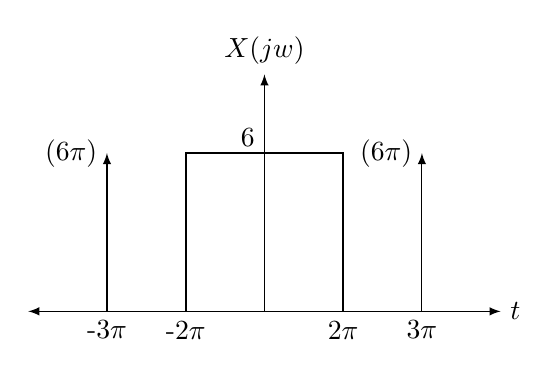
\begin{tikzpicture}
    \def\x{1} % replace 1 with desired value here
    \draw[-latex] (0,0) -- ++(-3,0);
    \draw[-latex] (0,0) -- ++(3,0)  node[right]{$t$};
    \draw[-latex] (0,0) -- ++(0,3.0\x)node[above]{$X(jw)$};
    \draw[] (0,0) -- ++(0,2.2\x)node[left]{6};
    \draw[] (-2,0) -- ++(0,0)node[below]{-3$\pi$};
    \draw[] (2,0) -- ++(0,0)node[below]{3$\pi$};
    \draw[thick] (0,2.0\x)node[above]{} -- ++(1,0) -- ++(0,-2.0\x)node[below]{2$\pi$};
    \draw[thick] (0,2.0\x)node[above]{} -- ++(-1,0) -- ++(0,-2.0\x)node[below]{-2$\pi$};
    \draw[-latex] (2,0) -- ++(0,2.0\x)node[left]{$(6\pi)$};
    \draw[-latex] (-2,0) -- ++(0,2.0\x)node[left]{$(6\pi)$};
  \end{tikzpicture}
  .\\\\\\   
      \end{enumerate}


\item 
    \begin{enumerate}
    \item %write the solution of q4a
        $ X_{p}(e^{jw}) = \dfrac{1}{T}  \mathlarger{\sum_{k=-\infty}}^{\infty}X(j(w-\pi k))$\\\\\\
        $X_{d}$(n) = $X_{p}$(j$\dfrac{w}{T}$)\\\\\\
        $ X_{d}(e^{jw}) = \dfrac{1}{2}  \mathlarger{\sum_{k=-\infty}^{\infty}} \dfrac {2w}{\pi}-\pi k$ \hspace{1cm} $|$w$| \leq \dfrac{\pi}{2}$ \\\\\\
         
   
        
    
    \item %write the solution of q4b
    
    
    $ H(e^{jw}) = \pi (\delta(w + \pi) + \delta(w - \pi)) $ \\\\\\
    
    \newpage
    \item %write the solution of q4c
    $ Y_{d}(e^{jw}) = X_{d}(e^{jw})*H(e^{jw})$\\\\\\
    $ Y_{d}(e^{jw}) = \dfrac{1}{2}  \mathlarger{\sum_{k=-\infty}^{\infty}} [\dfrac {2w}{\pi}-\pi k] * [\pi (\delta(w + \pi) + \delta(w - \pi))] $\\\\\\
    $ Y_{d}(e^{jw}) = \dfrac{\pi}{2}  \mathlarger{\sum_{k=-\infty}^{\infty}} \dfrac {2(w + \pi)}{\pi} + \dfrac {2(w - \pi)}{\pi} -2\pi k$
    

    \end{enumerate}



\end{enumerate}
\end{document}

